\begin{figure}[t]
\begin{center}
\begin{small}
\begin{tabular}{c@{\hskip2pt}c@{\hskip2pt}c@{\hskip2pt}c@{\hskip2pt}c}
Image&Target&Ours&AME&GlAtEx\\
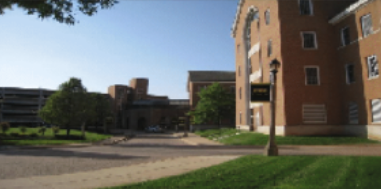
\includegraphics[width=\smallestimg,height=\smallestimg]{figures/seg_ade/1/img.png}&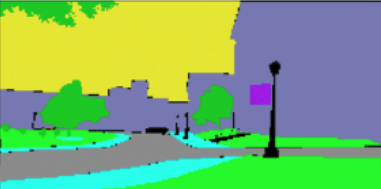
\includegraphics[width=\smallestimg,height=\smallestimg]{figures/seg_ade/1/gt.png}&
\includegraphics[width=\smallestimg,height=\smallestimg]{figures/seg_ade/1/ours.png}&
\includegraphics[width=\smallestimg,height=\smallestimg]{figures/seg_ade/1/ade.png}&
\includegraphics[width=\smallestimg,height=\smallestimg]{figures/seg_ade/1/glatex.png}\\

\includegraphics[width=\smallestimg,height=\smallestimg]{figures/seg_ade/2/img.png}&
\includegraphics[width=\smallestimg,height=\smallestimg]{figures/seg_ade/2/gt.png}&
\includegraphics[width=\smallestimg,height=\smallestimg]{figures/seg_ade/2/ours.png}&
\includegraphics[width=\smallestimg,height=\smallestimg]{figures/seg_ade/2/ade.png}&
\includegraphics[width=\smallestimg,height=\smallestimg]{figures/seg_ade/2/glatex.png}\\

\includegraphics[width=\smallestimg,height=\smallestimg]{figures/seg_ade/3/img.png}&
\includegraphics[width=\smallestimg,height=\smallestimg]{figures/seg_ade/3/gt.png}&
\includegraphics[width=\smallestimg,height=\smallestimg]{figures/seg_ade/3/ours.png}&
\includegraphics[width=\smallestimg,height=\smallestimg]{figures/seg_ade/3/ade.png}&
\includegraphics[width=\smallestimg,height=\smallestimg]{figures/seg_ade/3/glatex.png}\\

\includegraphics[width=\smallestimg,height=\smallestimg]{figures/seg_ade/4/img.png}&
\includegraphics[width=\smallestimg,height=\smallestimg]{figures/seg_ade/4/gt.png}&
\includegraphics[width=\smallestimg,height=\smallestimg]{figures/seg_ade/4/ours.png}&
\includegraphics[width=\smallestimg,height=\smallestimg]{figures/seg_ade/4/ade.png}&
\includegraphics[width=\smallestimg,height=\smallestimg]{figures/seg_ade/4/glatex.png}\\
\end{tabular}
\end{small}
\caption{\textbf{Segmentation qualitative results.} Sample semantic segmentation of our method compared with AME~\cite{pardyl2023active} and GlAtEx~\protect\cite{seifi2021glimpse} on the ADE20k dataset. In terms of quality, the segmentation maps generated by our approach are at least comparable to those produced by competing methods.}
\end{center}
\label{fig:qualiative-seg}
\end{figure}